\documentclass[12pt]{article}
\usepackage[letterpaper,margin=1in]{geometry}
\usepackage{amsmath,amssymb}
\usepackage{booktabs}
\usepackage{graphicx}
\usepackage{parskip}
\usepackage{float}
\usepackage[hidelinks]{hyperref}

\begin{document}

\begin{center}
{\LARGE\bfseries Final Benchmarks and Robustness of the\\[2pt] Graph-Laplacian Water-Quality Model\par}
\vspace{6pt}
{\large Where the River Network Helps, and Where It Does Not\par}
\vspace{14pt}
\hrule
\end{center}

\section{Summary}

This note collects the final results of the Graph-Laplacian model since the Nov 5 meeting. The full
analysis, with every table and caveat, is in \texttt{kron\_vs\_full\_laplacian\_report.pdf}.

\begin{itemize}
  \item With fair model selection for every model, the graph model is clearly best for
        \textbf{specific conductance} and \textbf{pH}. It ties with the linear models for water
        temperature and is mid-pack for dissolved oxygen (DO) and turbidity.
  \item Its advantage holds when several stations are held out at once, but \textbf{not} when a whole
        subbasin is held out. The graph model interpolates between stations of the same subbasin.
  \item Most model extensions did not help. The exception is the reading at neighbouring stations
        at the same hour, which clearly improves pH.
  \item Every model fails in the Lower Colorado, whose three stations all sit below large dams.
\end{itemize}

\section{The Model and the Graph}

For station $i$ and hour $t$ the model is
\[
  y_{i,t} = \beta_0 + X_{i,t}\beta + S_i\gamma + g_i + \varepsilon_{i,t},
\]
and the Graph-Laplacian model minimizes
\[
  \boxed{\;\sum_{i=1}^{m} \frac{1}{n_i} \sum_{t} \bigl(y_{i,t} - \beta_0 - X_{i,t}\beta - S_i\gamma - g_i\bigr)^2
  \;+\; \lambda_L\, g_B^{T} L_{\text{eff}}\, g_B \;+\; \lambda_\beta \bigl(\|\beta\|_2^2 + \|\gamma\|_2^2\bigr)\;}
\]
over $\beta_0$, $\beta$, $\gamma$ and $g_B$, subject to
\[
  \sum_{i=1}^{m} g_i = 0.
\]
Here,
\begin{itemize}
  \item $i = 1, \dots, m$ indexes the monitoring stations (graph nodes) in the training data, and
        $t$ the hours observed at station $i$;
  \item $y_{i,t}$ is the observed water-quality value (the target) at station $i$ and hour $t$;
  \item $X_{i,t}$ is the row of time-varying predictors: the other water-quality variables used
        for this target and the daily and annual Fourier terms;
  \item $S_i$ is the row of static MERIT Hydro covariates of station $i$ (elevation, log upstream
        area, log channel width, height above nearest drainage, local slope);
  \item $\beta_0$ is the intercept, and $\beta$ and $\gamma$ are the coefficient vectors of
        $X_{i,t}$ and $S_i$;
  \item $g_i$ is the station effect of station $i$: the station's offset that the predictors do not
        explain;
  \item $g_B = (g_1, \dots, g_m)^{T}$ is the vector of station effects at the retained monitoring
        nodes $B$;
  \item $\varepsilon_{i,t}$ is the residual error;
  \item $n_i$ is the number of hourly rows at station $i$; the factor $1/n_i$ gives every station
        the same total influence, as in the Oct 29 notes;
  \item $L_{\text{eff}} = L_{BB} - L_{BI} L_{II}^{-1} L_{IB}$ is the $m \times m$ Kron-reduced
        Laplacian of the Nov 5 notes \cite{dorfler}, with $L$ the weighted Laplacian of the river
        network and $I$ its interior nodes;
  \item $\lambda_L \ge 0$ controls how strongly the station effects are smoothed over the network;
        a large $\lambda_L$ pulls connected stations' effects together;
  \item $\lambda_\beta \ge 0$ is the ridge penalty on $\beta$ and $\gamma$ (the intercept $\beta_0$
        is not penalized), and $\|\cdot\|_2$ is the Euclidean norm;
  \item the constraint $\sum_i g_i = 0$ keeps the station effects from absorbing the intercept.
\end{itemize}
The Laplacian weighting, $\lambda_L$, $\lambda_\beta$ and the feature set (which columns of
$X_{i,t}$ and $S_i$ are used) are chosen by the inner leave-one-station-out loop.

The river network is built from MERIT Hydro \cite{merit}. In the uncompressed graph every grid
cell of about 90\,m is a node, linked to the next cell downstream: 67{,}401 nodes and 67{,}400 edges,
forming a tree (Figure~\ref{fig:uncompressed}). All but 66 of these nodes are pass-through cells with
one cell upstream and one downstream; the rest are station cells, confluences, sources and the
outlet.

\begin{figure}[tbp]
\centering
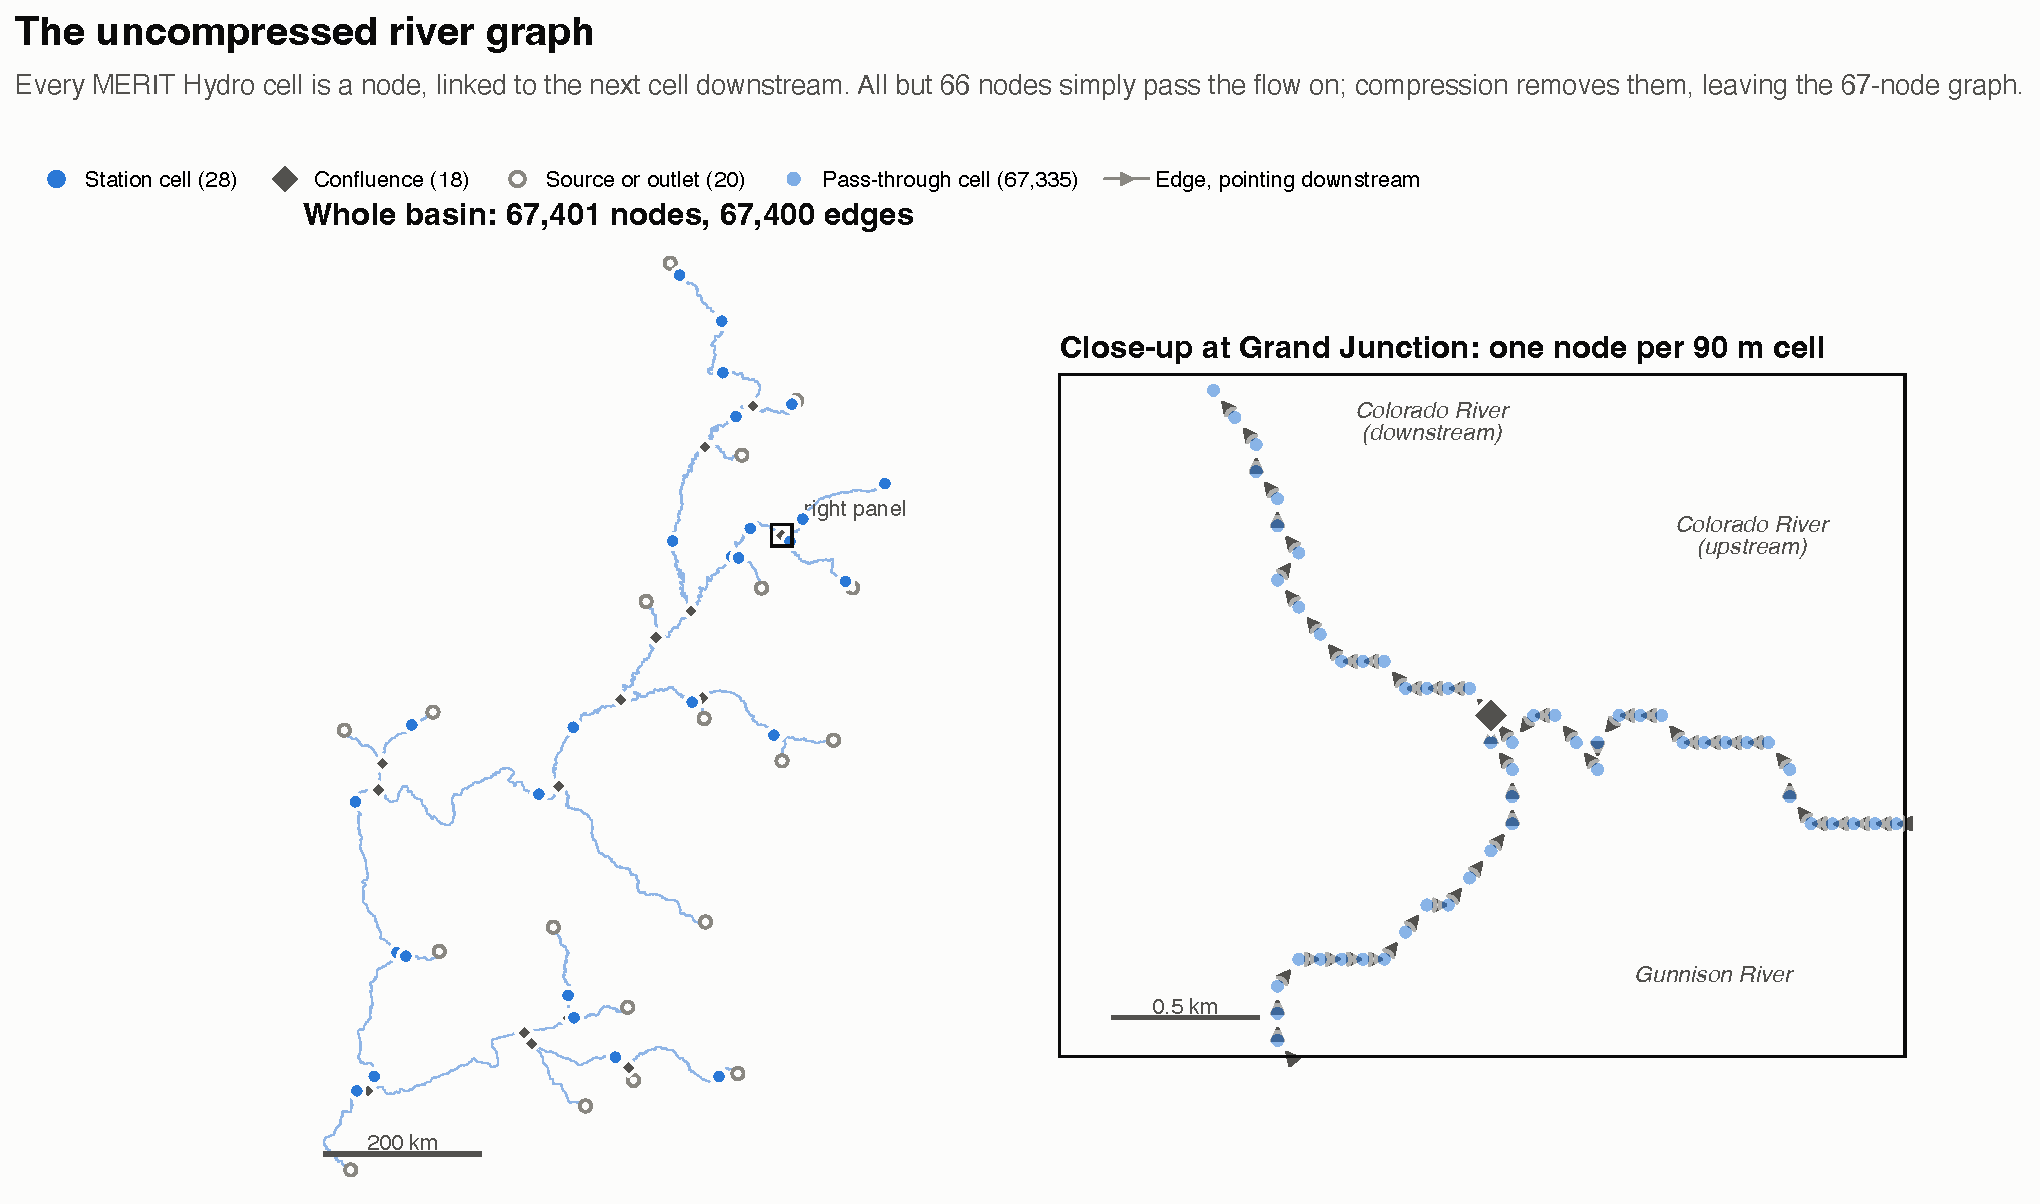
\includegraphics[width=\textwidth]{figures/poster_6_uncompressed.pdf}
\caption{The uncompressed graph: the whole basin (left) and a close-up of the Gunnison confluence
at Grand Junction (right), where each dot is one 90\,m cell and each arrow an edge pointing
downstream.}
\label{fig:uncompressed}
\end{figure}

Compression keeps only stations, confluences and river ends as nodes. Every chain of pass-through
cells between two nodes becomes one edge, weighted by its length (Figure~\ref{fig:graph}). The
result has 67 nodes and 66 edges, of which 26 nodes hold water-quality stations.

\begin{figure}[tbp]
\centering
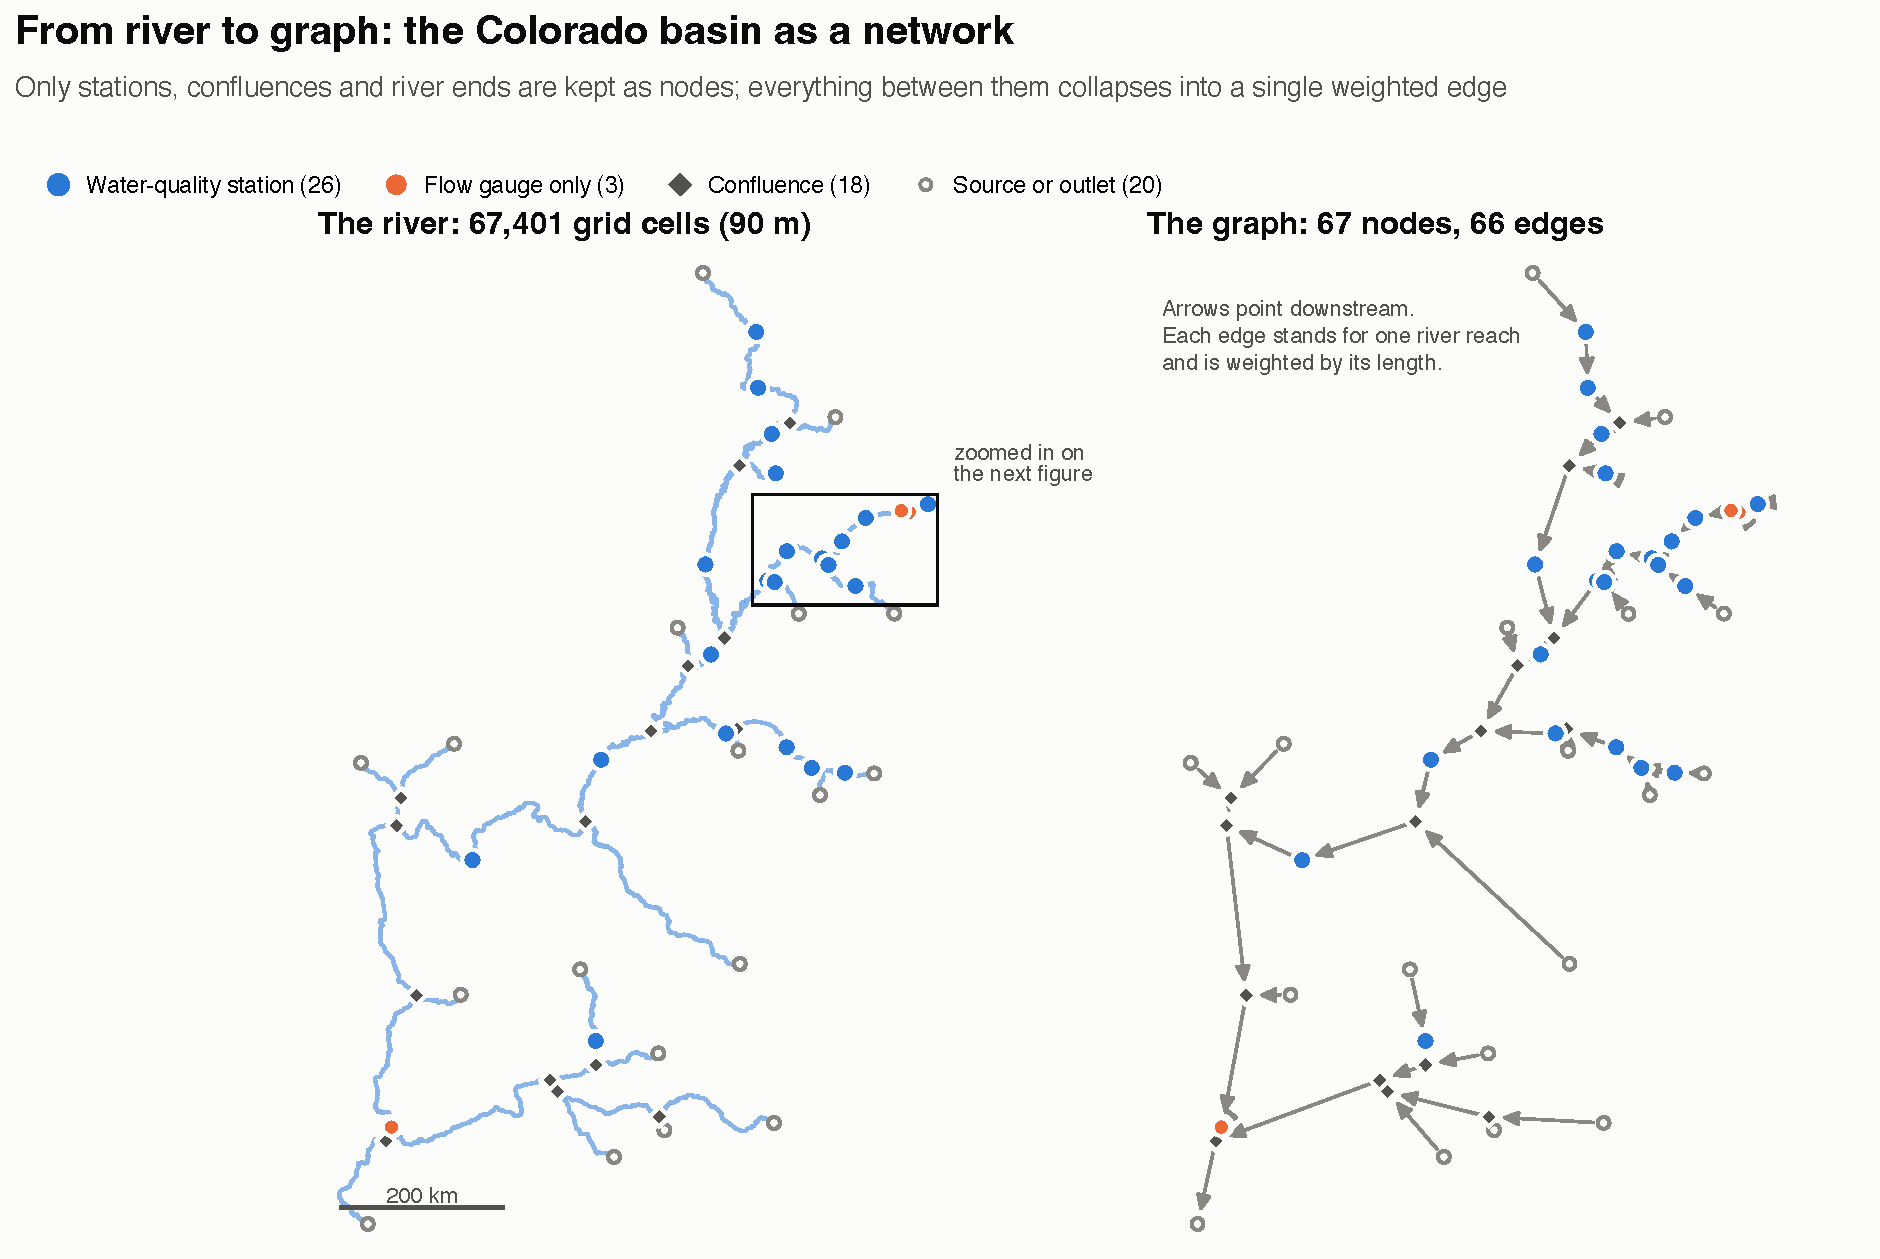
\includegraphics[width=0.92\textwidth]{figures/poster_4_graph.pdf}
\caption{The river network (left) and the graph built from it (right).}
\label{fig:graph}
\end{figure}

\begin{figure}[tbp]
\centering
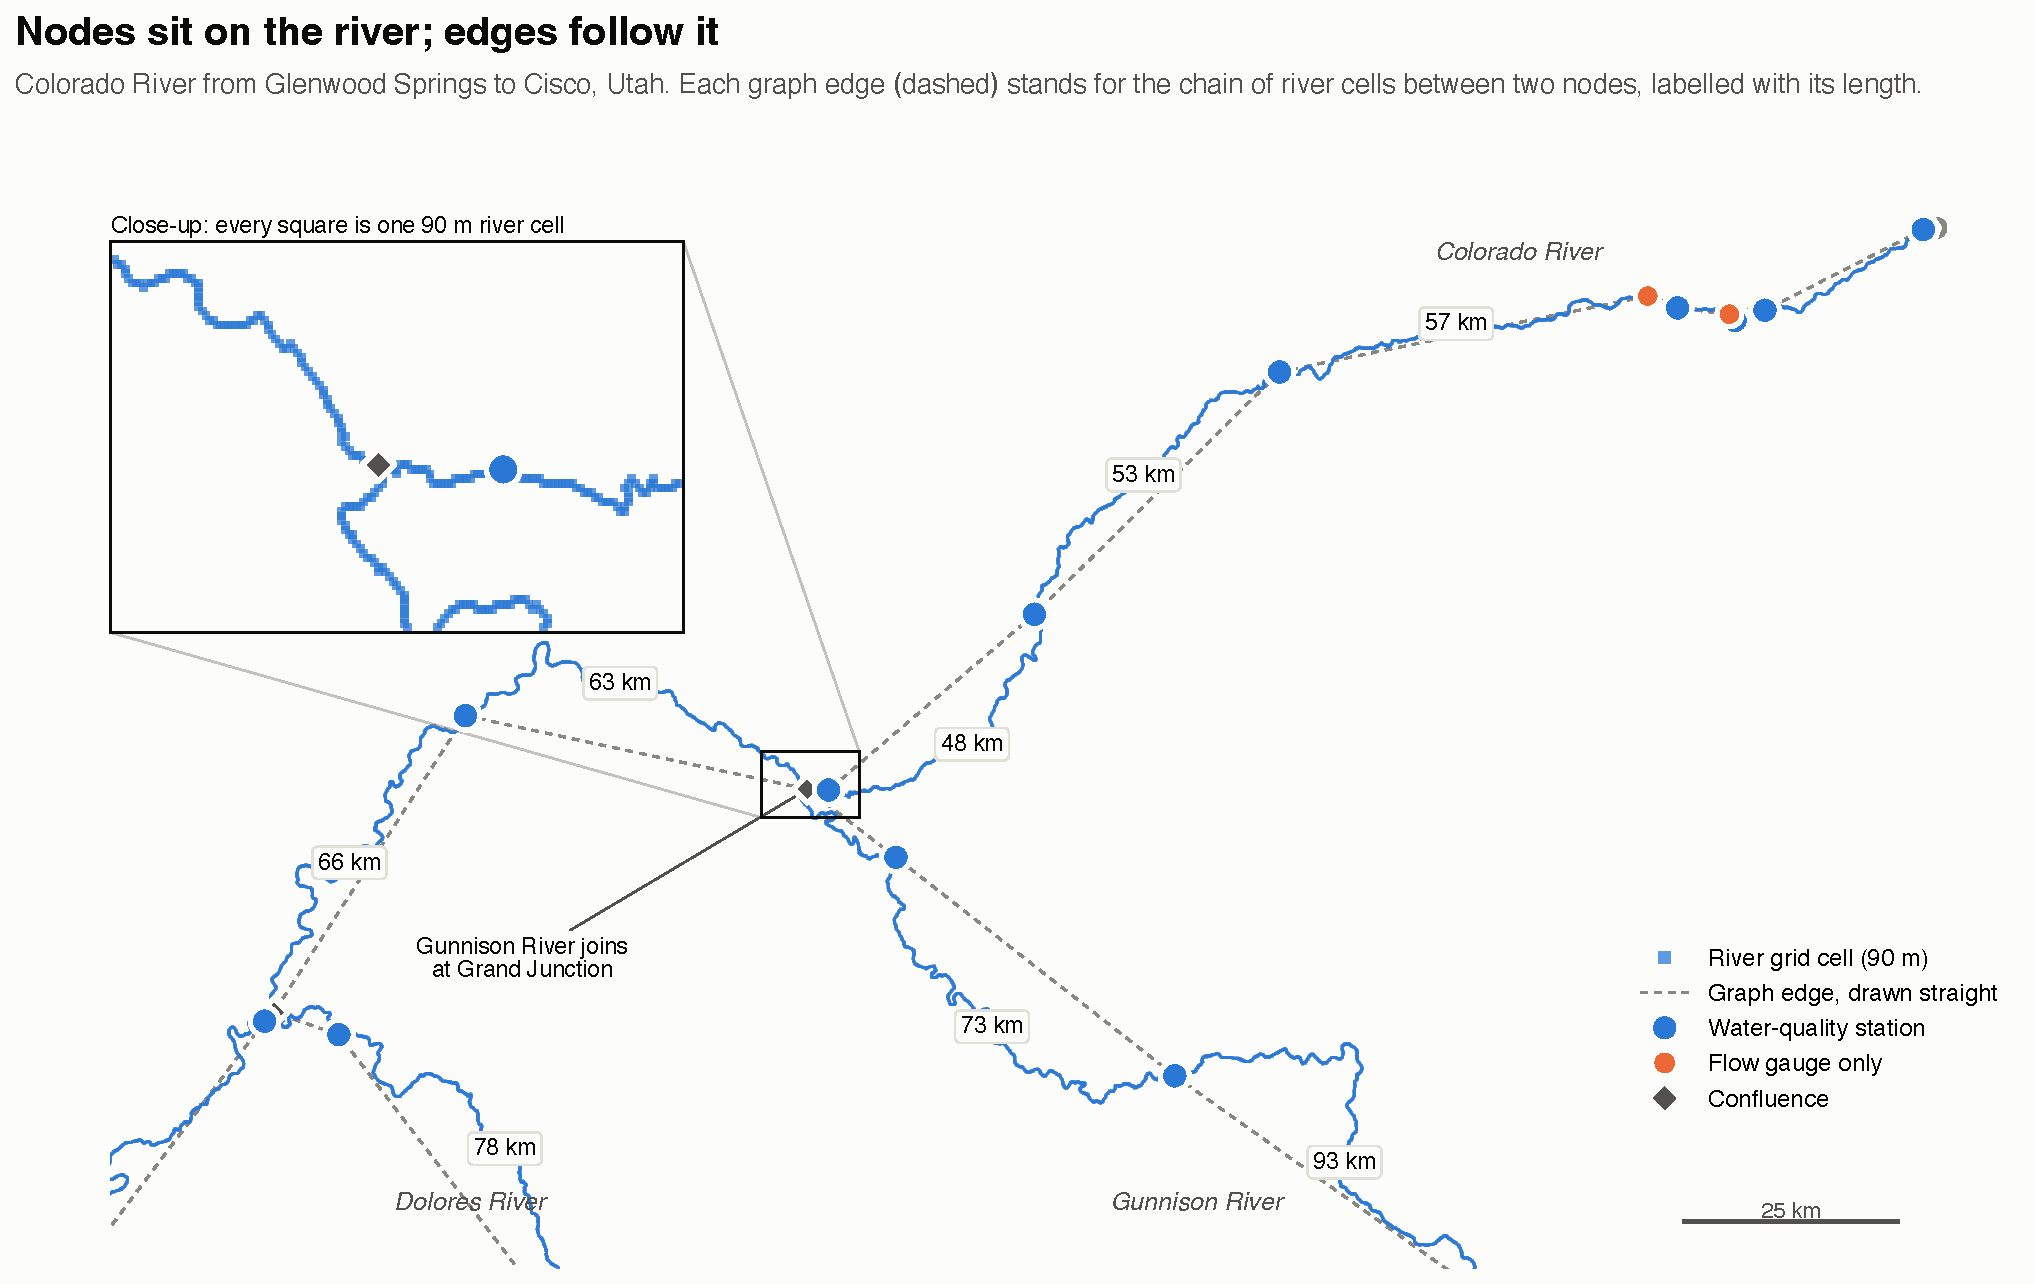
\includegraphics[width=0.92\textwidth]{figures/poster_5_zoom.pdf}
\caption{Close-up of the Colorado River from Glenwood Springs to Cisco, Utah. Each edge stands for
the river cells between two nodes.}
\label{fig:zoom}
\end{figure}

Kron reduction is exact for this model. It matches the full 67{,}401-node Laplacian to rounding
error, gives identical hyperparameters and $R^2$, and is about $150\times$ faster.

\section{Final Benchmark}

All results use leave-one-station-out (LOO) prediction, as on Nov 5. Unlike the Nov 5 table,
every model now chooses its features and settings in an \emph{inner} leave-one-station-out loop on
the training stations only. The held-out station is never used to choose anything.

\begin{table}[H]
\centering
\caption{Final LOO benchmark ($R^2$, equal station weights). Best in bold.}
\label{tab:final}
\begin{tabular}{l rrrrr}
\toprule
Model & Water temp. & DO & Spec.\ cond. & pH & Turbidity \\
\midrule
Stations           & 24 & 17 & 24 & 19 & 17 \\
\midrule
\textbf{Graph-Laplacian} & 0.8634 & 0.6996 & \textbf{0.3847} & \textbf{0.1173} & 0.1043 \\
OLS                & 0.8634 & 0.6951 & $-0.0987$ & $-0.0138$ & 0.1360 \\
Ridge              & \textbf{0.8640} & 0.7008 & $-0.1096$ & 0.0029 & 0.1362 \\
Elastic Net        & 0.8635 & 0.7048 & $-0.1089$ & 0.0226 & 0.1362 \\
Spline GAM         & 0.8382 & 0.7076 & 0.0218 & 0.0117 & 0.0910 \\
Random Forest      & 0.7579 & 0.6845 & $-0.1740$ & $-0.2685$ & 0.0996 \\
Gradient Boosting  & 0.8326 & \textbf{0.7327} & $-0.0939$ & $-0.1713$ & \textbf{0.3911} \\
Dummy (mean)       & $-0.0327$ & $-0.0286$ & $-0.0623$ & $-0.0301$ & $-0.0271$ \\
\bottomrule
\end{tabular}
\end{table}

\textbf{Specific Conductance.} The graph model is the only model that predicts unseen stations
usefully:
\[
  R^2:\quad 0.022 \;\longrightarrow\; 0.385
\]
from the best other model (Spline GAM) to the graph model. Fair selection first lowered the Nov 5
value ($0.253$) to $0.207$. An unweighted Laplacian on the compressed graph (one step per reach),
chosen by the inner loop, then raised it to $0.385$.

\textbf{pH.} The graph model is the only model meaningfully above zero:
\[
  R^2:\quad 0.023 \;\longrightarrow\; 0.117.
\]

\textbf{Water Temperature and DO.} Seasonality and water temperature explain most of the
variation. The graph model ties with the linear models for water temperature and is within $0.033$
of gradient boosting for DO.

\textbf{Turbidity.} Gradient boosting leads by a wide margin ($0.391$). No additive model,
including the graph model, captures turbidity's nonlinear response.

\subsection{What Changed Since Nov 5}

The graph model's $R^2$ moved in two steps (Table~\ref{tab:nov5}).

\begin{table}[H]
\centering
\caption{Graph-Laplacian LOO $R^2$ in the Nov 5 notes, with fair (inner-loop) selection of features
and settings, and in the final model, which adds the unweighted compressed Laplacian as a candidate.}
\label{tab:nov5}
\begin{tabular}{l rrr}
\toprule
Target & Nov 5 notes & Fair selection & Final \\
\midrule
Water temperature    & 0.8628 & 0.8628 & 0.8634 \\
DO                   & 0.7261 & 0.6998 & 0.6996 \\
Specific conductance & 0.2525 & 0.2068 & \textbf{0.3847} \\
pH                   & 0.1316 & 0.1299 & 0.1173 \\
Turbidity            & 0.0145 & 0.1063 & 0.1043 \\
\bottomrule
\end{tabular}
\end{table}

\begin{enumerate}
  \item \textbf{Fair selection.} On Nov 5 every model used a fixed, hand-picked feature set, partly
        designed with the leave-one-out results in view. Choosing the features inside the inner
        loop lowered the graph model's specific conductance from $0.253$ to $0.207$ and DO from
        $0.726$ to $0.700$. Turbidity rose ($0.015 \to 0.106$) because the inner loop could choose
        richer seasonal terms, which helped almost every model.
  \item \textbf{The unweighted network.} The final model adds one more candidate weighting: every
        reach of the compressed graph counts as one step, whatever its length. The inner loop chose
        it in all 24 folds for specific conductance, raising $R^2$ from $0.207$ to $0.385$. pH kept
        mostly the distance weighting, and the other targets changed by less than $0.002$.
\end{enumerate}

On the compressed graph every edge is a whole reach between stations, confluences and river ends.
Counting reaches rather than kilometres says that two stations are similar when few confluences
separate them. A plausible reason this suits salinity, not tested here, is that it changes mostly
where tributaries of different chemistry join.

\subsection{What the Graph Term Contributes}

Removing one variable at a time from the model shows what each target depends on
(Table~\ref{tab:ablation}).

\begin{table}[H]
\centering
\caption{Ablation: change in LOO $R^2$ when one variable is removed from the graph model (a
separate run with each target's fixed chemistry predictors; the full-model $R^2$ is in the first
row). Large negative values are variables nothing else can replace.}
\label{tab:ablation}
\begin{tabular}{l rrrr}
\toprule
Variable removed & Water temp. & DO & Spec.\ cond. & pH \\
\midrule
\emph{Full model}   & \emph{0.860} & \emph{0.722} & \emph{0.315} & \emph{0.131} \\
\midrule
Graph term          & $0.000$  & $-0.008$ & $\mathbf{-0.449}$ & $\mathbf{-0.109}$ \\
Annual cycle        & $\mathbf{-0.721}$ & $-0.010$ & $-0.107$ & $-0.035$ \\
Daily cycle         & $-0.009$ & $-0.116$ & $+0.003$ & $-0.043$ \\
Water temperature   & --       & $\mathbf{-0.211}$ & $+0.025$ & -- \\
Elevation           & $-0.030$ & $-0.032$ & $-0.042$ & $0.000$ \\
Local slope         & $-0.039$ & $-0.006$ & $-0.150$ & $-0.026$ \\
\bottomrule
\end{tabular}
\end{table}

\begin{itemize}
  \item The \textbf{graph term} is the most valuable input for specific conductance and pH, and
        adds nothing for water temperature and DO.
  \item \textbf{Water temperature} is driven by the annual cycle, and \textbf{DO} by water
        temperature and the daily cycle (photosynthesis).
  \item Among the MERIT Hydro covariates only local slope consistently helps.
\end{itemize}

\begin{figure}[tbp]
\centering
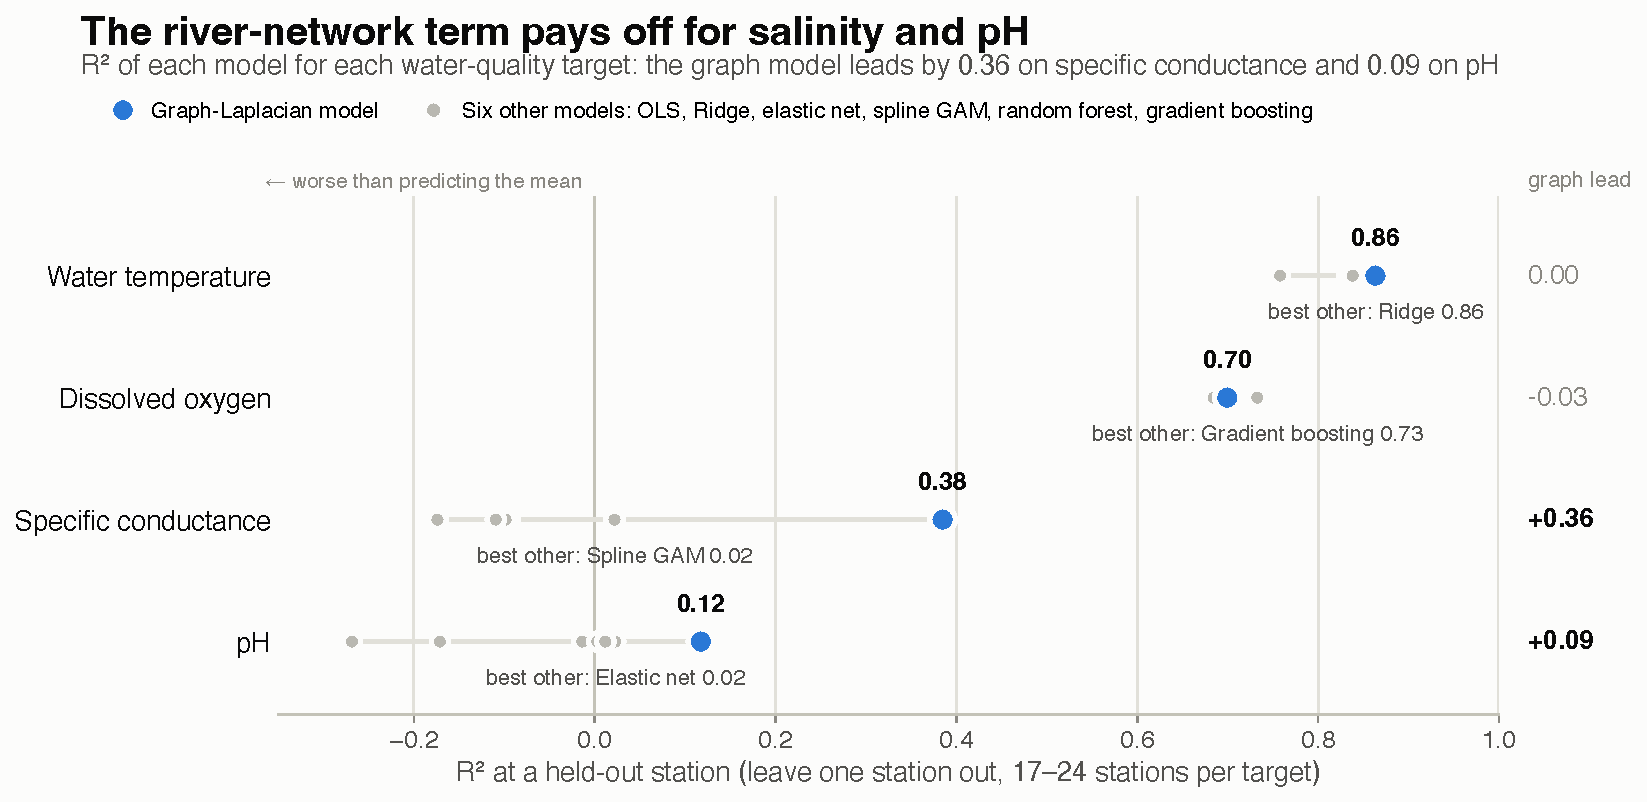
\includegraphics[width=\textwidth]{figures/poster_1_models.pdf}
\caption{LOO $R^2$ of the graph model (blue) and the six other models (grey).}
\label{fig:models}
\end{figure}

\section{Extensions That Did Not Help}

Each extension was offered to the inner loop as an extra option and compared with the final model
on identical rows (Table~\ref{tab:ext}).

\begin{table}[H]
\centering
\caption{Change in the graph model's LOO $R^2$ from each extension. With 17--24 stations,
changes below about $0.03$ are noise. The station-bootstrap 95\% interval excludes zero only where
marked $^{*}$.}
\label{tab:ext}
\begin{tabular}{l rrrr}
\toprule
Extension & Water temp. & DO & Spec.\ cond. & pH \\
\midrule
Other weights and settings & $+0.000$ & $+0.003$ & $-0.034$ & $+0.008$ \\
Dams as resistances        & $-0.001$ & $+0.014^{*}$ & $0.000$ & $+0.006$ \\
Tail-up covariance         & $0.000$  & $-0.007$ & $-0.227$ & $+0.004$ \\
REML settings              & $0.000$  & $+0.015$ & $-0.153^{*}$ & $-0.115^{*}$ \\
Network-varying annual cycle & $-0.022$ & $-0.015$ & $-0.005$ & $-0.002$ \\
Upstream geology, crop land & $0.000$ & $-0.002$ & $-0.019$ & $0.000$ \\
Graph + gradient boosting  & $-0.018$ & $-0.009$ & $-0.015$ & $+0.051$ \\
\bottomrule
\end{tabular}
\end{table}

\begin{itemize}
  \item \textbf{Other edge weights and settings} (confluence counts, length powers, log target,
        wider $\lambda$ grid): no gain; specific conductance $-0.034$.
  \item \textbf{Dams as high-resistance edges}: no gain for water temperature or turbidity.
  \item \textbf{Flow-directed (tail-up) covariance} \cite{verhoef}: specific conductance $-0.23$.
  \item \textbf{REML} choice of settings: worse for specific conductance and pH.
  \item \textbf{Discharge} as a predictor: no reliable change for the graph model.
  \item \textbf{Upstream-watershed geology and crop land} (EPA StreamCat \cite{streamcat}):
        specific conductance $-0.019$. The network already carries this information.
  \item \textbf{Graph + gradient boosting hybrid}: raised turbidity to $0.349$ under LOO, but on a
        later time period it was never better than the graph model alone and clearly worse for pH,
        so it is not adopted.
\end{itemize}

\section{Robustness to the Evaluation Split}

LOO holds out one station at a time, so a test station's neighbours are always in training. Three
further splits test how much the results depend on that.
\begin{itemize}
  \item \textbf{3 stations out}: 20 random draws of 20\% of the stations, tested together.
  \item \textbf{Subbasin out}: each of five subbasins (Colorado headwaters, Gunnison, Green, San
        Juan, Lower Colorado) held out whole.
  \item \textbf{Later period}: trained before 2026-01-01, tested on the other stations after it.
\end{itemize}

\begin{table}[H]
\centering
\caption{$R^2$ of the graph model, with the best other model in parentheses. The later-period run
compared only Ridge and gradient boosting with the graph model.}
\label{tab:splits}
\begin{tabular}{l cccc}
\toprule
Split & Water temp. & DO & Spec.\ cond. & pH \\
\midrule
LOO            & 0.863 (0.864) & 0.700 (0.733) & \textbf{0.385} ($0.022$)  & \textbf{0.117} ($0.023$) \\
3 stations out & 0.859 (0.861) & 0.702 (0.746) & \textbf{0.258} ($-0.060$) & \textbf{0.047} ($0.010$) \\
Subbasin out   & 0.851 (0.852) & 0.623 (0.709) & $-0.241$ ($-0.144$) & $-0.119$ ($-0.011$) \\
Later period   & 0.774 (0.760) & 0.543 (0.683) & \textbf{0.089} ($-0.116$) & $-0.136$ ($-0.022$) \\
\bottomrule
\end{tabular}
\end{table}

\begin{figure}[tbp]
\centering
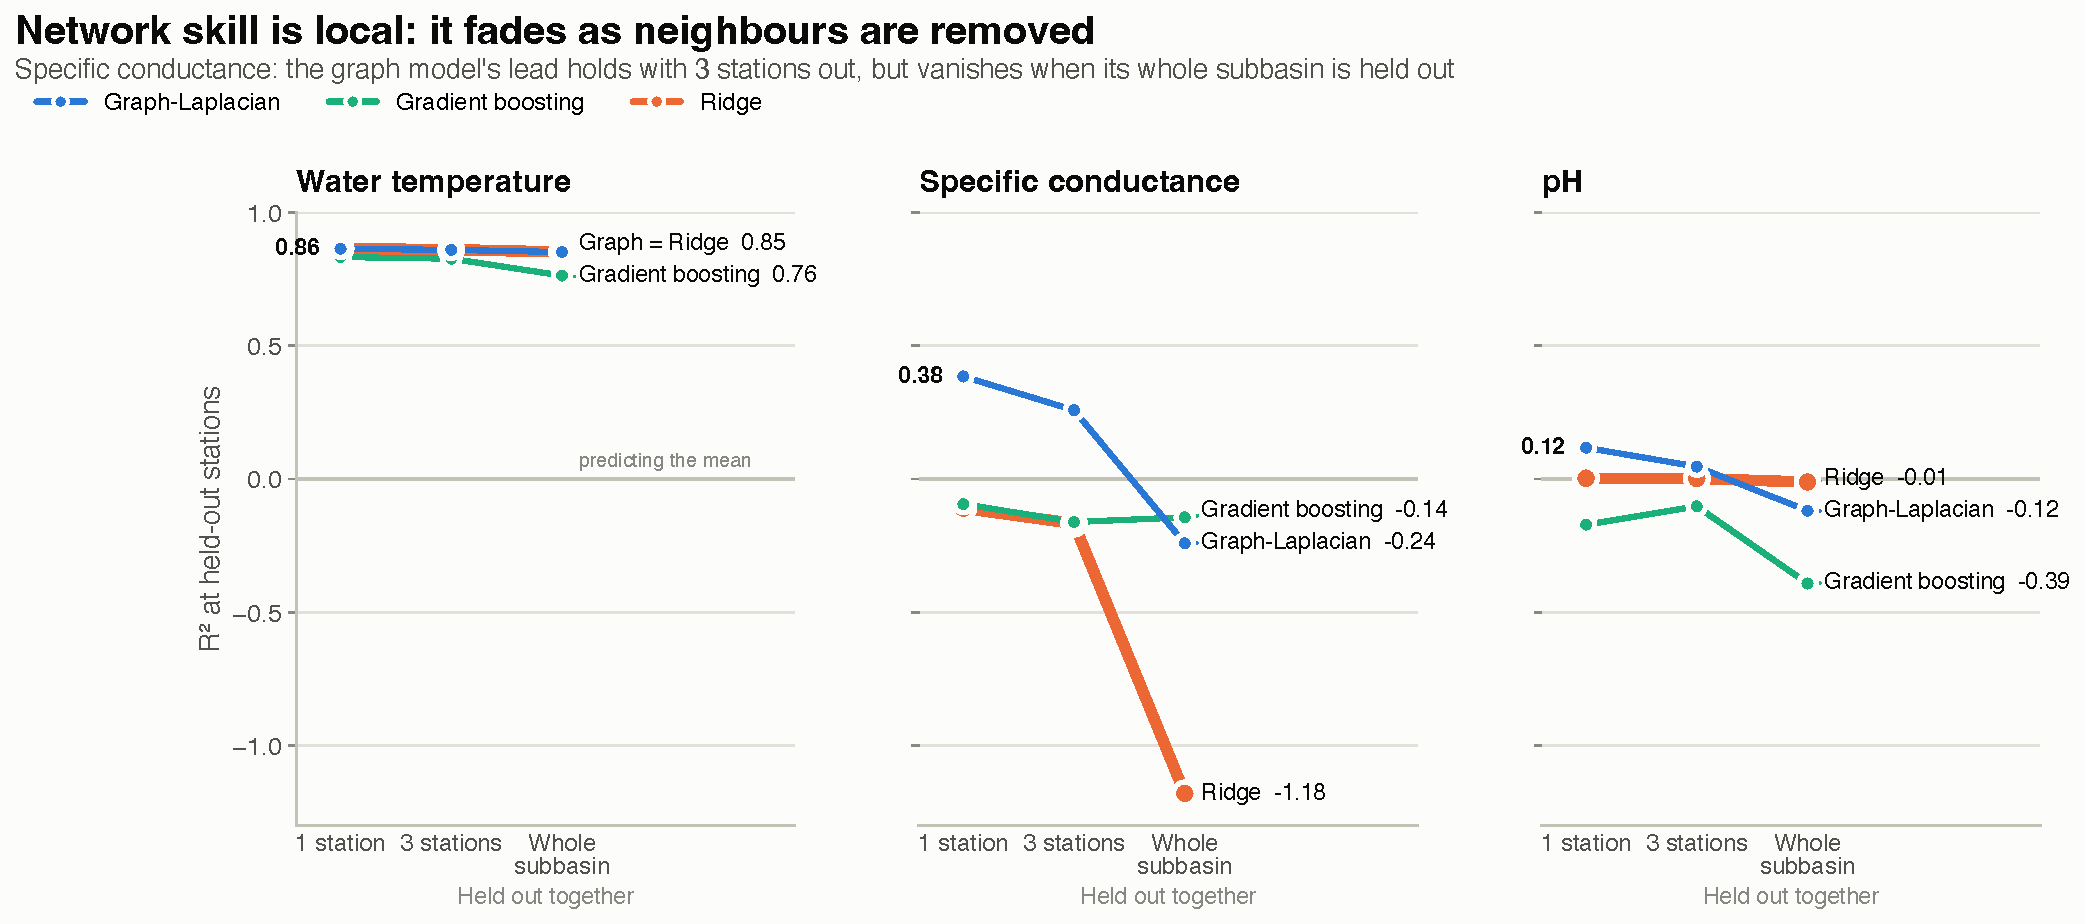
\includegraphics[width=\textwidth]{figures/poster_2_splits.pdf}
\caption{$R^2$ as more of the network is held out.}
\label{fig:splits}
\end{figure}

\textbf{Water temperature} transfers well under every split: it follows climate and season, which
all subbasins share.

\textbf{Specific conductance} keeps its lead with three stations out and on a later period, but
\[
  R^2:\quad 0.385 \;\longrightarrow\; -0.241
\]
when the whole subbasin is held out. The graph model then does worse than predicting the training
mean. Its skill is therefore interpolation from other stations of the same subbasin. It does not
carry a salinity level into a subbasin with no monitored station.

\textbf{pH} follows the same pattern on a smaller scale. On a later period every model is below zero.

\section{Where in the Basin the Model Works}

Grouping the LOO predictions by subbasin shows where each model works
(Tables~\ref{tab:sub_wt}--\ref{tab:sub_ph} and Figure~\ref{fig:map}). Within a subbasin, $R^2$ is
measured against that subbasin's own mean, so it is lower than the pooled values. The best of the
three models is in bold; ties at two decimals are broken by the unrounded value.

\begin{table}[H]
\centering
\small
\caption{LOO $R^2$ for water temperature within each subbasin.}
\label{tab:sub_wt}
\begin{tabular}{l c rrr}
\toprule
Subbasin & Stations & Graph & Ridge & Grad.\ boosting \\
\midrule
Colorado headwaters          & 7 & $0.94$ & $0.94$ & $\mathbf{0.95}$ \\
Green                        & 6 & $0.86$ & $0.86$ & $\mathbf{0.86}$ \\
Gunnison + Colorado--Dolores & 5 & $0.88$ & $0.88$ & $\mathbf{0.95}$ \\
San Juan                     & 3 & $0.87$ & $0.87$ & $\mathbf{0.87}$ \\
Lower Colorado + Verde       & 3 & $0.20$ & $\mathbf{0.20}$ & $-0.65$ \\
\bottomrule
\end{tabular}
\end{table}

\begin{table}[H]
\centering
\small
\caption{LOO $R^2$ for DO within each subbasin.}
\label{tab:sub_do}
\begin{tabular}{l c rrr}
\toprule
Subbasin & Stations & Graph & Ridge & Grad.\ boosting \\
\midrule
Colorado headwaters          & 7 & $0.75$ & $0.76$ & $\mathbf{0.77}$ \\
Green                        & 2 & $0.86$ & $0.81$ & $\mathbf{0.95}$ \\
Gunnison + Colorado--Dolores & 4 & $0.83$ & $0.82$ & $\mathbf{0.86}$ \\
San Juan                     & 1 & $0.76$ & $0.89$ & $\mathbf{0.94}$ \\
Lower Colorado + Verde       & 3 & $\mathbf{-0.37}$ & $-0.41$ & $-0.45$ \\
\bottomrule
\end{tabular}
\end{table}

\begin{table}[H]
\centering
\small
\caption{LOO $R^2$ for specific conductance within each subbasin.}
\label{tab:subbasin}
\begin{tabular}{l c rrr}
\toprule
Subbasin & Stations & Graph & Ridge & Grad.\ boosting \\
\midrule
Colorado headwaters          & 7 & $\mathbf{0.52}$ & $-0.17$ & $-0.19$ \\
Green                        & 6 & $\mathbf{0.37}$ & $-0.88$ & $-1.98$ \\
Gunnison + Colorado--Dolores & 5 & $\mathbf{0.11}$ & $-0.30$ & $-0.23$ \\
San Juan                     & 3 & $\mathbf{-0.79}$ & $-6.99$ & $-5.14$ \\
Lower Colorado + Verde       & 3 & $\mathbf{-0.52}$ & $-1.03$ & $-0.72$ \\
\bottomrule
\end{tabular}
\end{table}

\begin{table}[H]
\centering
\small
\caption{LOO $R^2$ for pH within each subbasin.}
\label{tab:sub_ph}
\begin{tabular}{l c rrr}
\toprule
Subbasin & Stations & Graph & Ridge & Grad.\ boosting \\
\midrule
Colorado headwaters          & 6 & $\mathbf{0.16}$ & $-0.00$ & $-0.07$ \\
Green                        & 2 & $\mathbf{-0.06}$ & $-0.57$ & $-1.18$ \\
Gunnison + Colorado--Dolores & 4 & $\mathbf{0.15}$ & $-0.08$ & $-0.08$ \\
San Juan                     & 4 & $-0.08$ & $-0.05$ & $\mathbf{0.30}$ \\
Lower Colorado + Verde       & 3 & $\mathbf{-0.27}$ & $-0.40$ & $-2.70$ \\
\bottomrule
\end{tabular}
\end{table}

\begin{figure}[tbp]
\centering
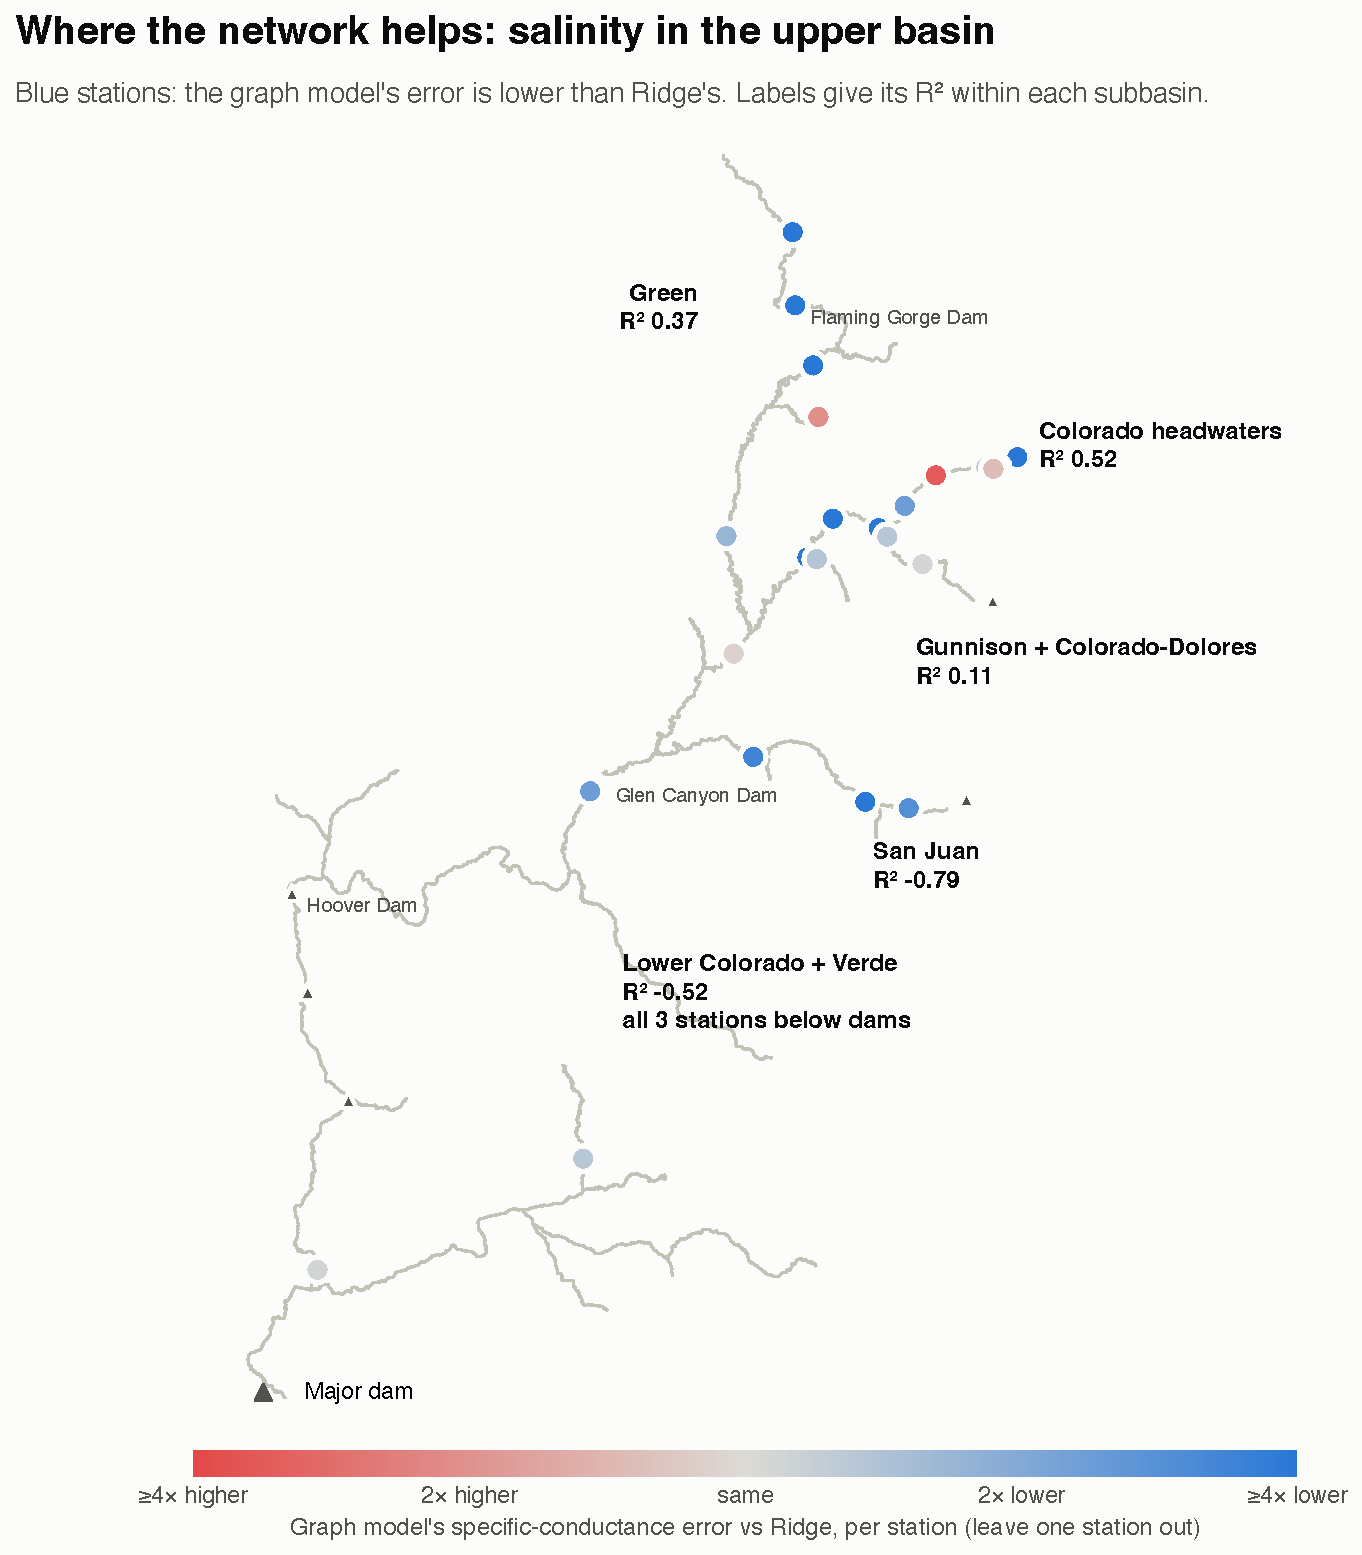
\includegraphics[width=0.52\textwidth]{figures/poster_3_map.pdf}
\caption{Graph-model specific conductance error relative to Ridge at each station (blue: lower).}
\label{fig:map}
\end{figure}

\begin{itemize}
  \item \textbf{Water temperature} is predicted well ($0.86$--$0.95$) in every subbasin except the
        Lower Colorado. The three models are within $0.07$ of each other.
  \item \textbf{DO}: gradient boosting is best in four of five subbasins, by $0.01$ to $0.18$ over
        the graph model (the largest gap at the single San Juan station).
  \item \textbf{Specific conductance}: only the graph model is positive in any of these subbasins,
        all three in the upper basin, where Ridge and gradient boosting are negative. Holding a
        subbasin out removes exactly these neighbours (Section~5).
  \item \textbf{pH}: the graph model is best in four of five subbasins. Gradient boosting is best
        in the San Juan ($0.30$).
\end{itemize}

The \textbf{Lower Colorado} fails for every target and every model, even water temperature (best
$0.20$). Its three stations are all tailwaters of large dams (Lees Ferry below Glen Canyon Dam,
the Verde below Bartlett Dam, and above Imperial Dam). Releases of deep reservoir water mute the
annual cycle that the seasonal terms expect: the median within-record standard deviation of water
temperature is $2.5$\,\textdegree C there, against $5.7$--$6.5$\,\textdegree C elsewhere.

\subsection{Upper-Basin Stations Only}

Table~\ref{tab:regions} scores the same LOO predictions on subsets of the stations. The models are
not refitted. Each $R^2$ is pooled over the stations of the subset, with equal station weights.

\begin{table}[H]
\centering
\small
\caption{LOO $R^2$ of the graph model on station subsets, with the best other model in
parentheses. Station counts in brackets. The Upper Colorado Basin is every subbasin above Lees
Ferry, i.e.\ all but the Lower Colorado.}
\label{tab:regions}
\resizebox{\textwidth}{!}{%
\begin{tabular}{l cccc}
\toprule
Stations included & Water temp. & DO & Spec.\ cond. & pH \\
\midrule
All stations          & 0.863 (0.864) [24] & 0.700 (0.733) [17] & \textbf{0.385} (0.022) [24] & \textbf{0.117} (0.023) [19] \\
Excl.\ San Juan and Lower Colorado & 0.900 (0.923) [18] & 0.796 (0.831) [13] & \textbf{0.381} ($-0.003$) [18] & \textbf{0.216} (0.082) [12] \\
Upper Colorado Basin  & 0.899 (0.918) [21] & 0.795 (0.840) [14] & \textbf{0.425} (0.027) [21] & \textbf{0.140} (0.076) [16] \\
Colorado headwaters only & 0.937 (0.952) [7] & 0.753 (0.775) [7] & \textbf{0.521} (0.269) [7] & \textbf{0.161} (0.056) [6] \\
\midrule
Lower Colorado only      & 0.202 (0.203) [3] & $-0.368$ ($-0.407$) [3] & $-0.520$ ($-0.107$) [3] & $-0.273$ ($-0.397$) [3] \\
\bottomrule
\end{tabular}}
\end{table}

\begin{itemize}
  \item \textbf{Specific conductance and pH}: the graph model stays clearly first in every subset except the Lower Colorado,
        reaching $0.42$--$0.52$ and $0.14$--$0.22$ in the upper basin.
  \item \textbf{Water temperature and DO} rise for every model once the Lower Colorado tailwaters
        are left out ($0.86 \to 0.90$ and $0.70 \to 0.80$). Gradient boosting then leads by
        $0.02$--$0.05$.
  \item Leaving out the San Juan barely changes specific conductance ($0.385 \to 0.381$), although
        the graph model is negative within it. Its stations widen the spread between stations,
        which the graph model largely captures.
  \item \textbf{Lower Colorado only}: every model is below zero except for water temperature
        (about $0.20$), and none beats the training mean for specific conductance ($-0.088$). The
        graph model is the least poor for DO and pH.
  \item These subsets were chosen after seeing the results, so they describe where the model
        works; they are not an independent test. A fair upper-basin-only result would need the
        models refitted and validated on those stations alone.
\end{itemize}

\section{Neighbouring Stations Help pH}

One extension did help: the anomaly of the three nearest training stations at the same hour
(Table~\ref{tab:nbr}).

\begin{table}[H]
\centering
\caption{Change in LOO $R^2$ when the neighbour reading is offered to the inner loop (paired, same
rows). $^{*}$: the station-bootstrap 95\% interval excludes zero. Last column: pH $R^2$ with it.}
\label{tab:nbr}
\begin{tabular}{l rrrr r}
\toprule
Model & Water temp. & DO & Spec.\ cond. & pH & pH $R^2$ \\
\midrule
Graph-Laplacian & $+0.010$ & $+0.012$ & $+0.007$ & $+0.061$ & \textbf{0.178} \\
OLS             & $+0.011$ & $+0.006$ & $+0.059^{*}$ & $+0.143^{*}$ & 0.130 \\
Ridge           & $+0.011$ & $+0.004$ & $+0.049^{*}$ & $+0.118^{*}$ & 0.121 \\
Elastic Net     & $+0.011$ & $+0.016$ & $+0.049^{*}$ & $+0.121^{*}$ & 0.143 \\
Spline GAM      & $+0.004$ & $-0.009$ & $-0.002$ & $+0.141^{*}$ & 0.153 \\
\bottomrule
\end{tabular}
\end{table}

\begin{itemize}
  \item \textbf{pH}: every conventional model gains $0.12$--$0.14$ (intervals above zero), and the
        graph model rises from $0.117$ to $0.178$, the best LOO pH so far.
  \item \textbf{Specific conductance}: the linear models gain about $0.05$; the graph model barely
        changes.
  \item Water temperature and DO gain about $0.01$; turbidity falls slightly.
\end{itemize}
This feature needs live readings from neighbouring stations, so it answers a different question:
filling in an unmonitored site while its neighbours report.

\section{Conclusions and Next Steps}

\begin{itemize}
  \item The Graph-Laplacian model is the model to use for \textbf{specific conductance} and
        \textbf{pH} at unmonitored sites, provided the subbasin has monitored stations.
  \item For water temperature and DO, simple linear models are just as good. For turbidity,
        gradient boosting is best.
  \item Claims should be limited to interpolation within monitored subbasins. Predicting an
        unmonitored subbasin is not supported.
  \item \textbf{Running:} the model with the longer record back to October 2020 (about $5\times$ the
        rows), and gradient boosting with the neighbour reading.
  \item \textbf{Proposed:} a dam-tailwater indicator, or a weaker seasonal cycle below major dams,
        for the Lower Colorado stations.
\end{itemize}

{\small
\begin{thebibliography}{9}
\bibitem{dorfler} F. D\"orfler and F. Bullo, ``Kron Reduction of Graphs With Applications to
  Electrical Networks,'' \emph{IEEE Transactions on Circuits and Systems I: Regular Papers}, vol.~60,
  no.~1, pp.~150--163, 2013, doi: 10.1109/TCSI.2012.2215780.
\bibitem{merit} D. Yamazaki, D. Ikeshima, J. Sosa, P. D. Bates, G. H. Allen, and T. M. Pavelsky,
  ``MERIT Hydro: A High-Resolution Global Hydrography Map Based on Latest Topography Dataset,''
  \emph{Water Resources Research}, vol.~55, pp.~5053--5073, 2019.
\bibitem{verhoef} J. M. Ver Hoef, E. Peterson, and D. Theobald, ``Spatial Statistical Models That
  Use Flow and Stream Distance,'' \emph{Environmental and Ecological Statistics}, vol.~13, no.~4,
  pp.~449--464, 2006.
\bibitem{streamcat} R. A. Hill, M. H. Weber, S. G. Leibowitz, A. R. Olsen, and D. J. Thornbrugh,
  ``The Stream-Catchment (StreamCat) Dataset: A Database of Watershed Metrics for the Conterminous
  United States,'' \emph{Journal of the American Water Resources Association}, vol.~52, no.~1,
  pp.~120--128, 2016.
\end{thebibliography}
}

\end{document}
